\documentclass[acmsmall,screen,review,anonymous]{acmart}


\usepackage{enumitem}
\usepackage{booktabs}
\usepackage{multirow}
\usepackage{amsmath}
\usepackage{amsfonts}
\usepackage{tabularx}
\usepackage{graphicx}
\usepackage{float}
\graphicspath{{figures/}}
\usepackage{tikz}
\usepackage{pgfplots}
\pgfplotsset{compat=1.18}
\usepgfplotslibrary{groupplots}
\usepackage{pgf-pie}
\usetikzlibrary{shapes,arrows,positioning,calc}

\usepackage{xspace}

\newcommand{\tool}{\textsc{NormCoRe}\xspace}

\newcommand{\todo}[1]{\textcolor{red}{#1}}
\newcommand{\hkf}[1]{\textcolor{blue}{#1}}


\title{\tool: Normalized and Conditional Token Reduction for Efficient LLM-Based Code Processing}




\begin{document}

\begin{abstract}
% !TeX root = ../main.tex


Large language models (LLMs) are increasingly used for code-related tasks, such as code generation, completion, and test generation. These tasks often incur substantial token costs because conventional programming languages are designed primarily for human reading and writing, and consequently contain syntactic, formatting, and structural information that may be redundant for LLM processing. Existing approaches reduce this overhead by heuristically defining concise syntax rules or mining frequently occurring patterns. However, frequency alone does not indicate whether a pattern is suitable for compression, and indiscriminate application of frequency-based rules can degrade downstream performance. We present \tool, a reversible code representation designed to reduce the token overhead of code language models. \tool organizes code compression into a unified \textit{Normalization \& Hybrid Idioms Shorthanding} framework. First, \textit{Normalization} leverages Python grammar and decoder state to normalize layout and structural information that can be deterministically recovered during decoding. Then, \textit{Hybrid Idioms Shorthanding} mines recurring code idioms at multiple granularities from the normalized representation and encodes them using compact symbols with typed captures. To avoid performance degradation from indiscriminate compression, \tool further introduces \textit{Conditional Attention}, which uses an offline model-derived signal to assess each eligible shorthand occurrence and selectively materialize it in compressed form, thereby incorporating model-level information into the compression process. Our evaluation shows that \tool reduces token consumption by up to 26.44\% among the evaluated modern code tokenizers. Downstream experiments demonstrate that code models can learn, generate, and use the \tool dialect, retaining performance close to the original Python surface in most evaluated backbone--task combinations while exposing a model-dependent gap on Mistral generation. Ablation and sensitivity studies further demonstrate the contributions of the individual components and the robustness of the selected parameters.

\end{abstract}

%%
%% The code below is generated by the tool at http://dl.acm.org/ccs.cfm.
%% Please copy and paste the code instead of the example below.
%%
\begin{CCSXML}
<ccs2012>
 <concept>
  <ccs_id>10010147.10010178.10010179.10010182</ccs_id>
  <concept_desc>Computing methodologies~Natural language generation</concept_desc>
  <concept_significance>500</concept_significance>
 </concept>
 <concept>
  <ccs_id>10011007.10011006.10011041</ccs_id>
  <concept_desc>Software and its engineering~Compilers</concept_desc>
  <concept_significance>300</concept_significance>
 </concept>
</ccs2012>
\end{CCSXML}

\ccsdesc[500]{Computing methodologies~Natural language generation}
\ccsdesc[300]{Software and its engineering~Compilers}

\keywords{Code Compression, Reversible Code Representation, Code Language Models, Normalization, Code Idioms, Model-Aware Compression, Conditional Attention, Python Dialect}

\maketitle

% !TeX root = ../main.tex

\section{Introduction}\label{sec:intro}


Large language models (LLMs) have become increasingly important for software engineering tasks, including code generation, code completion, test generation, and program repair~\cite{chen2021codex,liu2023repobench,lemieux2023codamosa,jimenez2024swebench}. These workloads increasingly require models to process source code at function, repository, and issue level~\cite{liu2023repobench,jimenez2024swebench}. Therefore, token consumption has become a practical concern, directly affecting inference cost, context utilization, and the amount of code that can be processed within a single interaction. Since LLMs operate on tokenized sequences, reducing the usage of tokens required for code representation can therefore improve both the cost-effectiveness and scalability of code-centered LLM applications.

However, programming languages were designed primarily for human developers rather than language models. Source code contains substantial syntactic and representational information that is useful for human comprehension but may be redundant for LLM processing. For example, indentation, delimiters, repeated keywords, verbose identifiers, and frequently recurring syntactic idioms can consume considerable token budgets without providing proportional semantic information. This observation motivates a fundamental question: \textit{Can source code be represented in a more compact form that preserves the information required by code language models while reducing token consumption?}



Several recent studies have explored this direction by introducing alternative code representations or token-reduction techniques~\cite{simpy2024, tokensugar2024}. A common strategy is to define concise syntax rules that replace verbose source-code constructs with shorter representations~\cite{simpy2024}. Another strategy is to mine recurring code patterns and replace them with compact symbols (e.g., shorthand)~\cite{tokensugar2024}. Although frequency provides a natural criterion for identifying compressible patterns, it does not necessarily indicate whether compressing a pattern is beneficial to an LLM. A pattern may occur frequently but still be important for the model to explicitly observe in its original form. Consequently, applying compression solely according to syntactic heuristics or pattern frequency may reduce token consumption at the cost of downstream model performance.



Therefore, we identify two challenges in token reduction. Challenge 1:
How to identify and normalize systematic structural redundancies in code into a
compact and recoverable representation? Challenge 2: How to identify
recurring but contributive tokens?
% We observe two recurring forms of redundancy in Python code. The first is structural information that can be recovered from the language grammar and decoding state, such as indentation, line organization, block boundaries, and selected delimiters. The second is repeated code idioms: multi-token expressions, calls, statements, and short blocks that share a stable structure while varying in identifiers, literals, or subexpressions. These two forms arise at different levels, but both can be represented more compactly without discarding the program-specific content needed to reconstruct executable code. This observation reveals a key tension in code representation: \textit{token efficiency and model utility are not necessarily aligned}. An effective representation should not simply minimize the number of tokens. It should selectively remove representational redundancy while preserving the information and patterns that a model relies on for understanding and generating code. Moreover, such a representation should remain reversible, because developers and software tools ultimately need to recover executable source code from the compressed representation. These requirements make code compression fundamentally different from conventional source-code minification: the objective is not merely to produce a shorter program, but to construct a compact representation that is both machine-effective and deterministically recoverable.}

% Prior work demonstrates the feasibility of this direction.
%  Lossy simplification methods instead remove elements considered less important~\cite{dietcode2022,slimcode2024,leancode2025}, which can be useful for code understanding but is harder to apply when the model must generate complete code that can be restored and executed. These studies establish that code can be shortened, but leave two connected questions: how should structural and idiomatic redundancy be organized within one reversible representation, and how should that representation account for the target model's existing knowledge?


To address these challenges, we present \tool, a reversible code representation designed for code language models. \tool provides a unified \textit{Normalization \& Hybrid Idioms Shorthanding} and \textit{Conditional Attention} for deciding whether an eligible shorthand occurrence should actually be compressed. Specifically, \textit{Normalization} leverages Python grammar and decoder state to identify representational elements whose original forms can be reconstructed without ambiguity. On top of the normalized representation, \tool introduces \textit{Hybrid Idioms Shorthanding} to capture recurring code idioms at multiple granularities. Rather than restricting compression to individual tokens or fixed syntactic constructs, it mines recurring patterns from the normalized code surface and represents them using compact symbols and typed captures. Besides, Conditional Attention uses an offline model-derived signal to estimate the suitability of compression at individual occurrences. It then selectively materializes the shorthand only when the occurrence satisfies the compression condition.


We evaluate \tool from three complementary perspectives. First, we measure its compression effectiveness and examine how many tokens can be eliminated across different configurations. \tool achieves up to 26.44\% token reduction among the evaluated modern code tokenizers. Second, we investigate whether the compressed representation remains useful to code language models. Our downstream experiments evaluate whether models can learn, generate, and use the \tool dialect, and compare their performance against the original Python surface. The results show that models operating on \tool can retain performance close to that obtained with the original representation despite substantially reduced token consumption. Third, we conduct ablation and sensitivity studies to understand the contributions of Normalization, Hybrid Idioms Shorthanding, and Conditional Attention, as well as the impact of key parameter choices.


In summary, we make the following contributions:



\begin{itemize}[leftmargin=*]
    \item We present \tool, a reversible code representation that reduces the token overhead of Python code while preserving deterministic recovery to the original source representation.
    \item We propose a unified \textit{Normalization \& Hybrid Idioms Shorthanding} framework that combines grammar-aware normalization with multi-granularity idiom compression using compact symbols and typed captures.
    \item We introduce \textit{Conditional Attention}, a model-aware compression mechanism that selectively applies shorthand based on an offline model-derived signal rather than frequency alone.
    \item We conduct extensive experiments demonstrating the token-reduction capability, downstream model compatibility, and component effectiveness of \tool, achieving up to 26.44\% token reduction among the evaluated modern code tokenizers while retaining downstream performance close to the original Python surface.
\end{itemize}

% !TeX root = ../main.tex

\section{Background}
\label{sec:bg}


\subsection{Efficiency in LLM-Based Code Processing}
\label{subsec:token_electricity}

% TODO： 这个部分讲：
% 1. 模型用于Code Processing：generation， etc
% 2. 模型产生的code，有很多token，具体，一个issue问题解决，可能需要XXX token
% 3. token有很多冗余的
% 4. 冗余token 的问题解决，可以提升推理速度，同时帮助节省多少多少token成本。

Large language models (LLMs) are now used for a wide range of code-processing tasks. At the function level, HumanEval asks a model to generate function implementations from signatures and docstrings~\cite{chen2021codex}, while CodaMosa uses language models to support test generation~\cite{lemieux2023codamosa}. At the repository level, RepoBench evaluates code completion that depends on information from other files~\cite{liu2023repobench}, and SWE-bench asks systems to resolve real GitHub issues by producing patches for existing repositories~\cite{jimenez2024swebench}. These tasks may require the model to process functions, interfaces, usage examples, tests, and dependencies distributed across multiple files.

The resulting token cost can be substantial. SWE-Effi evaluated software-engineering agents on 50 stratified SWE-bench Verified issues and reported that AutoCodeRover with Qwen3-32B processed an average of 55.5K input tokens and 20.4K output tokens per issue attempt. Under the same model, SWE-Agent processed 440.2K input tokens and 41.0K output tokens~\cite{fan2025sweeffi}. Thus, a single real-world issue attempt can involve tens or even hundreds of thousands of tokens, depending on the workflow. More tokens increase computation, memory use, latency, and serving cost, while also consuming space that could hold other useful repository context.

Source code is designed primarily for people to write, read, and maintain. It therefore contains indentation, line organization, delimiters, fixed syntactic forms, and recurring code idioms that improve human readability but can expand into multiple model tokens. Some of this information is predictable from the programming language grammar or repeats across programs, while identifiers, literals, and program-specific expressions carry less replaceable information. Treating all of these elements identically leaves recoverable redundancy in the model input.

A denser code representation can reduce this redundancy after the relevant context has been selected. Shorter representations lower the number of tokens processed during training and inference, reduce latency and computational cost, and leave more of the context window available for useful program information. These benefits, however, require the representation to preserve the structure and content needed to recover executable code and to remain learnable by the model. This motivates reversible token reduction designed specifically for generative code processing.

\subsection{Motivating Example}


% 第一段，讲核心相关工作simpy token sugar原理
% 第二段，引入normalized例子，告诉别人还有reduction空间
% 第三段，引入conditional例子，告诉别人如果不做conditional，效果会适得其反，影响LLM推理准确率

SimPy~\cite{simpy2024} and TokenSugar~\cite{tokensugar2024} demonstrate two complementary ways to shorten source code. SimPy redesigns the Python surface grammar to reduce layout, delimiters, and other fixed syntactic forms~\cite{simpy2024}, whereas TokenSugar replaces recurring multi-token code patterns with compact shorthand tokens~\cite{tokensugar2024}. Consider the following Python function:

\begin{center}
\setlength{\fboxsep}{6pt}
\fbox{%
  \begin{minipage}{0.88\columnwidth}
\ttfamily\small
def collect(items, errors):\\
\hspace*{1em}result = []\\
\hspace*{1em}for item in items:\\
\hspace*{2em}if item is None:\\
\hspace*{3em}errors.append(item)\\
\hspace*{3em}continue\\
\hspace*{2em}result.append(item)\\
\hspace*{1em}return result
  \end{minipage}%
}
\end{center}

Its indentation and block organization support human readability, while \texttt{errors.append(item)} and \texttt{result.append(item)} instantiate the same recurring call structure. The example therefore contains both grammar-level redundancy and repeated idiomatic structure.

\tool handles these two forms within a unified representation. Normalization converts indentation, line organization, block boundaries, and selected fixed syntax into a compact surface that can be reconstructed from Python grammar and decoder state. Program-specific content, including \texttt{items}, \texttt{errors}, \texttt{result}, and \texttt{item}, remains explicit. Hybrid Idioms Shorthanding then operates on this normalized surface. For example, the two calls can share one shorthand schema, written schematically as \texttt{<append>(receiver, argument)}, with their different receivers and arguments retained as captures. Normalization therefore not only reduces structural tokens directly, but also provides a stable surface on which recurring idioms can be collected and represented consistently.

A reversible codec could replace both eligible calls because either shorthand can be decoded correctly. However, this uniform policy assumes that the two occurrences are equally suitable for the target model. Their surrounding control flow and prediction contexts differ, so replacing them may impose different adaptation costs even though they use the same shorthand schema. Conditional Attention evaluates the occurrences separately. It may retain \texttt{errors.append(item)} in expanded form while encoding \texttt{result.append(item)} with the shorthand, or make the opposite decision, according to the model-derived signal. This example motivates occurrence-level selection: the codec determines which transformations are valid, while the model signal determines where an eligible transformation is applied.


\subsection{Compression Opportunities in Source Code}
\label{subsec:rationale}

To characterize the theoretical and practical boundaries of code compression, we analyze token composition across three diverse Python corpora: CodeSearchNet, our GitHub-Code-Clean corpus, and our curated high-quality repository corpus. We classify tokens into seven functional classes according to their roles in source text and the abstract syntax tree (AST), and organize them into three tiers with different compression opportunities and risks. Figure~\ref{fig:taxonomy} shows the aggregate distribution, and Table~\ref{tab:taxonomy} summarizes the role of each class.

\begin{figure}[!t]
  \centering
  \definecolor{taxblue}{HTML}{4E79A7}
  \definecolor{taxorange}{HTML}{F28E2B}
  \definecolor{taxgreen}{HTML}{59A14F}
  \definecolor{taxred}{HTML}{E15759}
  \definecolor{taxpurple}{HTML}{B07AA1}
  \definecolor{taxteal}{HTML}{76B7B2}
  \definecolor{taxyellow}{HTML}{EDC948}
  \begin{tikzpicture}[
    scale=0.78,
    every node/.style={font=\scriptsize},
    taxslice/.style={draw=white, line width=0.8pt}
  ]
    \pie[
      text=legend,
      hide number,
      sum=99.9,
      radius=1.65,
      rotate=90,
      style={taxslice},
      color={taxblue, taxorange, taxgreen, taxred, taxpurple, taxteal, taxyellow}
    ]{
      10.5/Layout (10.5\%),
      21.9/Punctuation (21.9\%),
      5.3/Comments (5.3\%),
      4.1/Keywords (4.1\%),
      4.4/Operators (4.4\%),
      29.5/Identifiers (29.5\%),
      24.2/Literals (24.2\%)
    }
    \fill[white] (0,0) circle (0.78);
    \node[align=center, font=\sffamily\scriptsize] at (0,0) {Token\\composition};
  \end{tikzpicture}
  \vspace{-5pt}
  \caption{Token taxonomy across the analyzed Python corpora. Tiers 1 and 2 are the primary compression targets, while Tier 3 carries program-specific content.}
  \Description{Pie chart showing layout 10.5 percent, punctuation 21.9 percent, comments 5.3 percent, keywords 4.1 percent, operators 4.4 percent, identifiers 29.5 percent, and literals 24.2 percent.}
  \label{fig:taxonomy}
\end{figure}

\begin{table}[!t]
    \centering
    \footnotesize
    \setlength{\tabcolsep}{3pt}
    \renewcommand{\arraystretch}{1.05}
    \caption{Token taxonomy and aggregate distribution in the analyzed Python corpora.}
    \vspace{-5pt}
    \label{tab:taxonomy}
    % \begin{tabularx}{\columnwidth}{@{}llr>{\raggedright\arraybackslash}X@{}}

       \begin{tabular}{>{\raggedright\arraybackslash}p{1cm}
                >{\centering\arraybackslash}p{3cm}
                >{\raggedright\arraybackslash}p{1cm}
                >{\centering\arraybackslash}p{5cm}
                }
    \toprule
    \textbf{Tier} & \textbf{Functional class} & \textbf{Ratio} & \textbf{Compression property} \\
    \midrule
    1 & Formatting and layout & 10.5\% & Reconstructable layout markers \\
      & Syntax punctuation & 21.9\% & Repeated syntactic delimiters \\
      & Comments & 5.3\% & Non-executable documentation \\
    \midrule
    2 & Keywords & 4.1\% & Predictable structural operations \\
      & Operators & 4.4\% & Recurring symbolic operations \\
    \midrule
    3 & Identifiers & 29.5\% & Program-specific names \\
      & Literals & 24.2\% & Program-specific values \\
    \bottomrule
    \end{tabular}
\end{table}

This distribution reveals a hierarchy of compressibility and associated risks:

\begin{enumerate}[leftmargin=*]
    \item \textbf{High-yield redundancy (Tier 1).} Layout, punctuation, and comments account for 37.7\% of the observed tokens. Much of this material supports human-readable presentation or repeats structural information that a deterministic decoder can reconstruct. It therefore offers the largest immediate opportunity, although not every token in the tier can be removed under a reversible contract.
    \item \textbf{Predictable semantic space (Tier 2).} Keywords and operators account for another 8.5\%. They frequently occur in rigid syntax and recurring idioms, such as \texttt{for \_ in range} and \texttt{if \_\_name\_\_ == "\_\_main\_\_"}, making complete multi-token structures suitable for fixed-vocabulary shorthands.
    \item \textbf{Sensitive logical payload (Tier 3).} Identifiers and literals account for 53.7\%. They carry program-specific names, values, and data-flow relationships. \tool therefore keeps them explicit unless a reversible pattern schema transports them as captures.
\end{enumerate}

\textbf{Compression opportunity bound.} Tiers 1 and 2 together occupy approximately 46.2\% of the analyzed token stream, giving a first-order upper bound near 46\% when identifiers and literals are left unchanged. This is an opportunity bound derived from token composition, not a claim that every tokenizer can realize a 46\% reduction. Some syntax must remain explicit or be re-encoded, comments may be preserved, and shorthand symbols, captures, and boundaries all consume tokens. The realized gain therefore depends on the tokenizer, corpus, registry size, and reversible representation cost.

We test this estimate in RQ1 by encoding real programs and counting them with the same tokenizer before and after encoding. Normalization shortens recoverable structure, while Hybrid Idioms Shorthanding replaces repeated patterns that remain on the normalized surface. The measurements therefore show how these two forms of reduction complement each other and how much compression they achieve in practice.

% !TeX root = ../main.tex

\section{Methodology}\label{sec:method}

\begin{figure*}[!t]
  \centering
  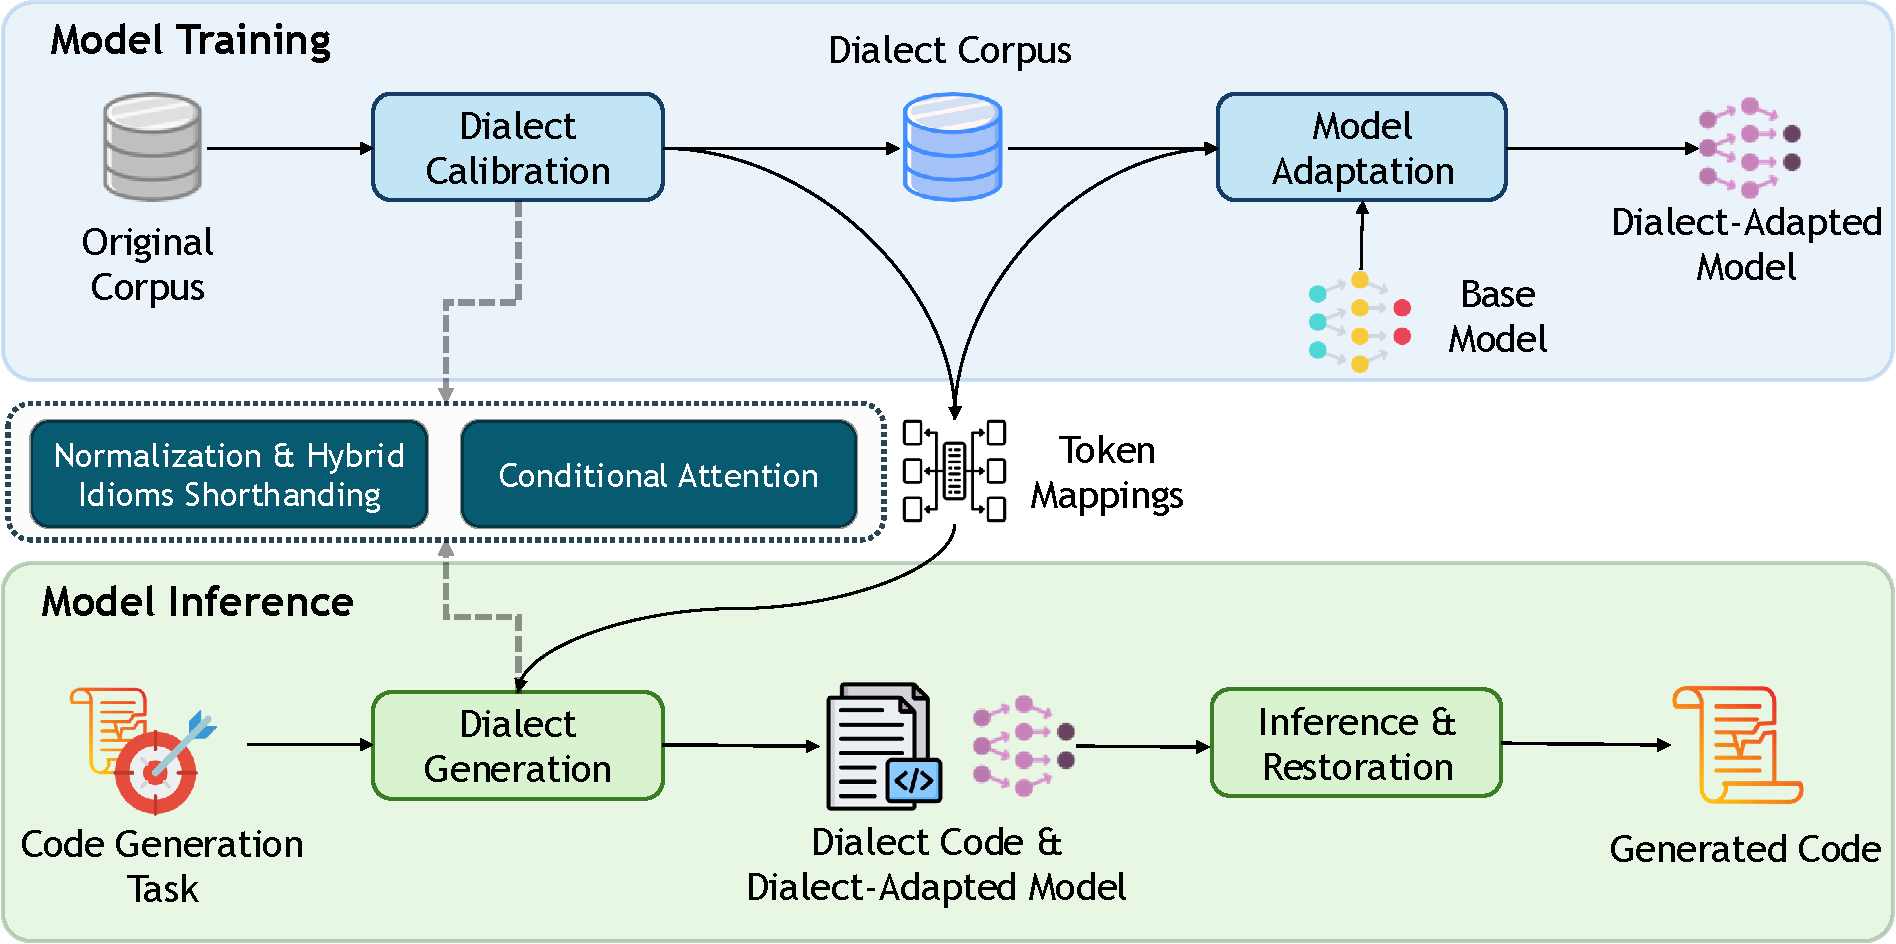
\includegraphics[width=0.8\textwidth]{NormCoRe-2.pdf}
  \vspace{-5pt}
  \caption{Overview of \tool}
  \Description{The NormCoRe workflow contains dialect calibration, model
  adaptation, and dialect-based inference. Calibration applies Normalization,
  Hybrid Idioms Shorthanding, and Conditional Attention; adaptation teaches a
  code model the resulting vocabulary and surface; inference restores generated
  dialect code to ordinary Python.}
  \label{fig:pipeline}
\end{figure*}




This section presents the \tool workflow, from constructing a reversible code dialect to adapting a model and restoring its generated code (Figure~\ref{fig:pipeline}).



\subsection{Overview}

% 介绍一下方法 model training ， model inference， dialect calibration model adaptation, dialect generation等，总体框架

\tool consists of three stages: dialect calibration, model adaptation, and dialect-based inference. Dialect calibration determines how ordinary Python is represented in a shorter but recoverable form. Model adaptation teaches a code model to read and generate that representation. During inference, the adapted model processes the calibrated dialect, and its output is restored to ordinary Python for execution or downstream use.

In \textbf{dialect calibration}, \tool first applies Normalization to compact layout and fixed syntactic structure that can be reconstructed from Python grammar and decoder state. It then collects recurring structures at multiple granularities and represents them through Hybrid Idioms Shorthanding. Fixed and corpus-mined idioms share one registry-based representation, while program-specific identifiers, literals, and expressions are retained directly or carried as captures. Conditional Attention further uses a signal from a reference code model to evaluate eligible shorthand occurrences in context, allowing the calibrated dialect to retain an expanded form where compression would be harder for the model to absorb.

In \textbf{model adaptation}, the shorthand symbols are added to the model vocabulary and the calibrated corpus is used for continued training. The symbols keep stable meanings throughout training, enabling the model to learn both the compact representation and its relationship to ordinary code. This stage turns the dialect from a codec-side transformation into a representation that the model can understand and generate.

In \textbf{dialect-based inference}, source context is encoded with the calibrated \tool representation and supplied to the adapted model. The model may then complete or generate code directly in the dialect. Finally, the reversible decoder expands shorthand symbols, restores normalized structure, and produces ordinary Python. These stages connect token reduction with model training and executable-code generation in one end-to-end workflow.



\subsection{Reversible Shorthanding}
\label{subsec:reversible_mapping}

\tool represents code as a compact textual dialect rather than as a binary compression stream. The dialect remains inside the language model's token space: ordinary program content is kept as code tokens, while recoverable structure and recurring idioms are expressed through a vocabulary of atomic symbols. The model can therefore consume and generate the compressed representation directly.

Let $x$ be a Python program. \tool first applies a deterministic normalization function $N$ that replaces recoverable layout and fixed syntactic structure with structural symbols. It then applies an idiom mapping $Q_{\mathcal{R}}$ defined by a registry $\mathcal{R}$. Each registry entry contains a pattern schema $P_i$, a shorthand symbol $S_i$, and an inverse template. For an occurrence with program-specific captures $c$, the mapping is
\begin{equation}
    P_i(c) \longleftrightarrow \langle S_i, c \rangle,
    \qquad S_i \in \mathcal{V}_{\mathrm{idiom}}.
\end{equation}
The captures carry the identifiers, literals, or expressions needed by that occurrence, so multiple concrete code spans can share one shorthand without discarding their differences. Together, the structural symbols used by $N$ and the idiom symbols used by $Q_{\mathcal{R}}$ form the added dialect vocabulary.

The complete encoder is $E_{\mathcal{R}}=Q_{\mathcal{R}}\circ N$. Its decoder reverses these operations: idiom symbols are expanded with their captures, and the normalized structure is reconstructed from the structural symbols and decoder state. The resulting program preserves the original syntax tree:
\begin{equation}
    \operatorname{AST}\!\left(D_{\mathcal{R}}(E_{\mathcal{R}}(x))\right)
    = \operatorname{AST}(x).
\end{equation}
This formulation provides a common reversible representation for both structural normalization and idiom shorthanding. The following subsections explain how \tool constructs this representation and how Conditional Attention decides where eligible idioms are materialized.

\subsection{Dialect Calibration and Generation}

\subsubsection{Normalization \& Hybrid Idioms Shorthanding}
\label{subsec:codec}

Dialect calibration constructs the representation that will be shared by the training corpus and the adapted model. \tool first applies Normalization to the input program. Guided by Python's concrete syntax and decoder state, it replaces recoverable indentation, line organization, block boundaries, and selected fixed syntax with structural symbols. Program-specific identifiers, literals, and expressions remain explicit. Besides reducing structural tokens directly, this step maps stylistically different programs onto a more regular surface for idiom collection.

Hybrid Idioms Shorthanding then collects recurring structures from the normalized corpus. The collector considers contiguous local windows and syntax-derived expression or statement spans, allowing it to represent idioms at multiple granularities. Exact patterns retain fully shared content, while generalized patterns replace varying identifiers, literals, or expressions with typed captures. Each selected schema is assigned an atomic shorthand symbol and an inverse template in the registry.

Pattern utility is measured on the complete shorthand representation under the target tokenizer, rather than by corpus frequency alone. For an occurrence $m$ of pattern $p$, let $z_m$ be its normalized span and let $g_p(c_m)$ contain the shorthand symbol and captures $c_m$. Its token saving is
\begin{equation}
    \Delta(m)=|T(z_m)|-|T(g_p(c_m))|,
\end{equation}
where $T$ is the target tokenizer. Occurrences with non-positive saving are discarded. The resulting registry therefore concentrates on idioms whose symbols still save tokens after their capture content is included.

Candidate occurrences may overlap. \tool treats them as weighted intervals and uses dynamic programming to select a non-overlapping set with maximum total saving:
\begin{equation}
    S^*=\arg\max_{S\ \mathrm{nonoverlap}}
    \sum_{m\in S}\Delta(m).
\end{equation}
The selected occurrences are materialized on the normalized surface using their shorthand symbols and captures. In this sense, dialect generation is an offline corpus transformation: it creates the compact code seen during model adaptation rather than adding another operation to autoregressive decoding.

Figure~\ref{fig:compression_examples} uses four labels for the granularities of
the mined examples. ``Layout and Structure'' denotes formatting and fixed
structural syntax that Normalization can reconstruct from grammar and decoder
state. ``Function Skeleton'' denotes a recurring function-definition shape
whose identifiers or expressions may vary. ``Multi-statement Span'' denotes a
contiguous recurring sequence containing more than one statement. ``Expression
and Call'' denotes a recurring expression-level or method-call idiom. In the
figure, ``Normalization'' is the normalized intermediate surface and ``Hybrid
Idioms'' is the shorthand surface in which registry symbols and typed captures
are materialized. These labels describe the scope of each example, not
additional compression algorithms.

\begin{figure*}[!t]
  \centering
  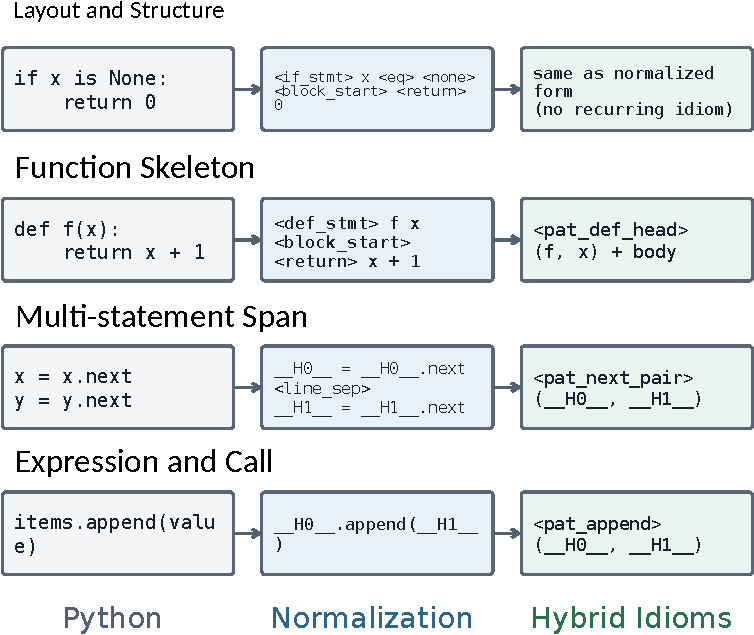
\includegraphics[width=0.7\textwidth]{NormCoRe_compression_examples_terms_cropped.pdf}
  \vspace{-5pt}
  \caption{Representative transformations in \tool. Normalization compacts recoverable layout and syntax, while Hybrid Idioms Shorthanding replaces recurring structures with registry symbols and typed captures. Program-specific content remains explicit or is carried by the captures.}
  \Description{Four examples show Python code transformed into a normalized structural dialect and then, where applicable, into a registry pattern with captures. The examples cover layout, function skeletons, multi-statement spans, and expressions or calls.}
  \label{fig:compression_examples}
\end{figure*}

\subsubsection{Conditional Attention}
\label{subsec:conditional_attention}

Not every legal occurrence of a shorthand imposes the same representation cost on a code model. The same idiom may appear in different control-flow and prediction contexts, and uniformly replacing every match ignores these differences. Conditional Attention therefore evaluates eligible occurrences individually while leaving the normalization rules, shorthand registry, and decoder unchanged.

For each occurrence $m$, \tool considers its expanded normalized context and a counterfactual context in which only that occurrence is replaced. A frozen reference model produces a contextual attention profile that summarizes how attention is allocated around the occurrence and how that allocation changes after replacement. This profile captures both the local importance of the original span and the response of its surrounding prediction context to the shorthand. We denote its standardized representation by $\mathbf{z}(m)$.

The contextual profile is calibrated against the local representation shift caused by the replacement. Let $y_m$ be a common suffix following the occurrence. We measure the change in its mean negative log-likelihood as
\begin{equation}
    d(m)=\operatorname{NLL}_{\mathcal{M}}(y_m\mid x_m^{\mathrm{short}})
         -\operatorname{NLL}_{\mathcal{M}}(y_m\mid x_m^{\mathrm{expanded}}).
\end{equation}
A positive value indicates that the shorthand makes the unchanged continuation harder for the reference model to predict. On a calibration split, \tool fits a regularized linear scorer
\begin{equation}
    \widehat d(m)=b+\mathbf{w}^{\top}\mathbf{z}(m)
\end{equation}
and then keeps the scorer fixed when constructing training or evaluation dialects.

To materialize a dialect at a chosen reduction level, eligible occurrences are ordered from the lowest to the highest predicted damage and admitted until the target number of token removals is reached. The admitted occurrences then enter the same non-overlapping selection used by Hybrid Idioms Shorthanding. Because the decision is occurrence-specific, two instances of the same registry pattern may be represented differently when their contexts produce different model responses. Conditional Attention is applied offline during dialect construction; it does not require an additional attention computation during model generation.

\subsection{Model Adaptation}

After dialect calibration, the structural symbols introduced by Normalization and the idiom symbols registered by Hybrid Idioms Shorthanding are added to the model vocabulary as atomic tokens. Source programs are transformed with the calibrated encoder, including the occurrence decisions made by Conditional Attention, to construct the dialect corpus used for adaptation. The meanings of these symbols remain consistent across the corpus: a structural symbol always represents the same recoverable syntax, and an idiom symbol always invokes the same registry schema and inverse template.

\tool adapts the model with the standard autoregressive language-modeling objective. For a materialized dialect sequence $\widetilde{x}=E_{\mathcal{R}}(x)$, the objective is
\begin{equation}
    \mathcal{L}_{\mathrm{adapt}}
    =-\sum_{t=1}^{|\widetilde{x}|}
    \log p_{\theta}(\widetilde{x}_t\mid \widetilde{x}_{<t}).
\end{equation}
No change to the model architecture or generation objective is required. Through continued training, the model learns how the added symbols interact with ordinary code tokens, how structural markers organize a program, and how shorthand symbols represent recurring code idioms. For symmetric dialect generation, both the context and target code use the \tool representation. When native output is preferred, the model can instead receive a condensed context while being supervised on ordinary Python targets.

\subsection{Inference and Restoration}

During dialect-based inference, the available source context is transformed with the same calibrated encoder used to prepare the training corpus. The adapted model then reads the shortened context and generates either \tool dialect code or native Python, according to the adaptation setting. Conditional Attention is part of dialect preparation and does not alter the model's autoregressive generation procedure.

For dialect output, restoration reverses the encoding stages in order. The decoder first expands each idiom symbol with its accompanying captures according to the registry template. It then restores the layout and fixed syntactic structure represented by the normalization symbols. The resulting ordinary Python program can be passed directly to existing parsers, execution environments, and software-engineering tools. In this way, token reduction remains internal to the model-facing representation, while the external interface continues to use standard source code.

% !TeX root = ../main.tex

\section{Experiments}
\label{sec:experiments}

We design the following research questions:

\begin{itemize}[leftmargin=*]
    \item \textbf{RQ1: Compression capability.} How much can \tool reduce token usage across Python corpora and tokenizers, and how do Normalization and Hybrid Idioms Shorthanding contribute to the gain?
    \item \textbf{RQ2: Dialect learnability and downstream use.} Can a code model learn and use the \tool dialect while retaining its capability on downstream software-engineering tasks?
    \item \textbf{RQ3: Conditional Attention.} At a comparable reduction level, can model-informed occurrence selection reduce the representation shift and adaptation cost introduced by Hybrid Idioms Shorthanding?
    \item \textbf{RQ4: Parameter sensitivity.} How sensitive is compression to the registry capacity and mining bounds, and which settings provide the best held-out operating point?
\end{itemize}

\subsection{Experimental Setup}
\label{subsec:data_setup}

We choose each corpus for a specific experimental role. CodeSearchNet (CSN) is collected from public GitHub repositories and covers diverse projects, APIs, and coding styles, making it suitable for testing compression on heterogeneous repository code~\cite{husain2019codesearchnet}. We use the Python subset of StarCoderData as the source of the continual-pretraining corpus in RQ2~\cite{starcoder2023,zhensuuu2024starcoderdata}. LeetCode contains compact function-level solutions with recurring algorithmic idioms; we use the publicly released \path{LeetCode_Python_Solutions_v2} collection for pattern mining~\cite{limyeri2024leetcode}. CodeContests provides problem-grouped solutions with many eligible pattern occurrences, enabling the controlled occurrence-level selection and problem-disjoint evaluation in RQ3~\cite{codecontests2022}. HumanEval is kept strictly for downstream evaluation because it is a widely used code-generation benchmark with function signatures, natural-language specifications, and executable tests for measuring functional correctness~\cite{chen2021codex}.

For RQ1, each corpus--tokenizer pair has a mining split and a disjoint evaluation split. Registries are mined independently for each pair, so RQ1 measures codec capacity under the corresponding tokenization and repetition distribution rather than the performance of one universal vocabulary. For RQ2, original-Python and \tool corpora are constructed from the same source documents, and one fixed multidomain registry is shared by all dialect samples. The same adapted checkpoint is used for code generation, completion, and test generation. For RQ3, we use a frozen candidate registry derived from CodeContests training problems. The Conditional Attention scorer is calibrated without access to the held-out problem groups and is compared with random occurrence selection at matched reduction levels. No evaluation benchmark is used for mining, calibration, or training.

Before materialization, sources are parsed, de-duplicated, and split by repository, or by problem for solution data. We remove overlap with held-out benchmarks and record the splits and codec configuration in reproducible manifests. Every dialect target is decoded and checked for executable, AST-equivalent recovery before use.

\subsection{Metrics and Evaluation Protocol}
\label{subsec:metrics}

All token counts use the same tokenizer before and after compression. For native token count $N$ and compressed wire count $C$, reduction is $1-C/N$. For RQ1 we report the aggregate ratio over a complete evaluation split, rather than the arithmetic mean of per-file percentages. The contributions of Normalization and Hybrid Idioms Shorthanding use the same native denominator. Structural and idiom symbols are counted as atomic special tokens, and capture parameters are included in the compressed representation.

For downstream tasks, we report Pass@1 and the realized reduction in model-facing tokens. In the symmetric dialect condition, the model receives and generates dialect code, and generated output is restored before execution. Compilation and strict restoration rates verify that the generated dialect remains usable. RQ3 measures local representation shift by the change in suffix negative log-likelihood (delta-NLL). It measures adaptation cost with validation NLL, perplexity, learning curves, and the number of steps required to reach a fixed loss threshold. In the RQ3 tables, ``Reduction (\%)'' is the fraction of all available candidate savings selected for a comparison, whereas ``Tokens removed'' is the corresponding absolute number of tokens; they describe the same reduction at relative and absolute scales.

\subsection{Model and Training Configuration}
\label{sec:setup}

RQ1 measures token counts with the tokenizers distributed with five exact checkpoints: Qwen2.5-Coder-1.5B~\cite{qwen2024}, DeepSeek-Coder-1.3B~\cite{deepseekcoder2024}, StarCoder2-3B~\cite{starcoder2_2024}, Mistral-7B~\cite{mistral2023}, and GPT-2~\cite{radford2019gpt2}. These names identify the tokenizer source; RQ1 does not run model inference.

The RQ2 dialect-absorption experiment uses Qwen2.5-Coder-1.5B as the
mainline backbone~\cite{qwen2024} and repeats the matched Baseline/\tool evaluation on
StarCoder2-3B~\cite{starcoder2_2024}, Mistral-7B~\cite{mistral2023}, and GPT-2~\cite{radford2019gpt2}. Each backbone uses a
LoRA parameter-efficient adapter~\cite{hu2022lora}, a fixed \tool vocabulary, matched source data,
and the same evaluation protocols for its two conditions. The Baseline condition uses the original Python surface; the \tool condition uses the calibrated dialect. All models are evaluated
on code generation, code completion, and reference-accepting test generation.

The RQ3 comparison uses the same backbone, tokenizer, codec, candidate registry, shared initialization, packed-data size, and optimizer configuration for both policies. Each policy is trained for 100 steps with sequence length 1024 and effective batch size 32. The only experimental variable is whether eligible shorthand occurrences are selected by Conditional Attention or by a reduction-matched random policy. Results are repeated across three training runs, while the occurrence-level test uses problem-disjoint calibration and evaluation splits.

% !TeX root = ../main.tex

\section{Evaluation}

\subsection{RQ1: Compression Capability}
\label{subsec:rq1_results}

We evaluate the codec across different Python corpora and tokenizers. Each \tool registry is mined from its corresponding training split and evaluated on disjoint code. We also run the released SimPy and TokenSugar implementations~\cite{simpy2024,tokensugar2024} on exactly the same held-out files. Table~\ref{tab:rq1_final} reports aggregate token counts and reductions measured with the same tokenizer before and after each encoding.

\begin{table*}[!t]
    \centering
    \scriptsize
    \setlength{\tabcolsep}{3.2pt}
    \renewcommand{\arraystretch}{1.08}
    \caption{RQ1 comparison on the same held-out inputs and tokenizers. $\mathrm{Tok}_b$ and $\mathrm{Tok}_a$ are the aggregate token counts before and after encoding, and ``Redu.'' is $100(1-\mathrm{Tok}_a/\mathrm{Tok}_b)$.}
    \vspace{-5pt}
    \label{tab:rq1_final}
    \resizebox{\textwidth}{!}{%
    \begin{tabular}{@{}llrrr|rrr|rrr@{}}
    \toprule
    \multirow{2}{*}{\textbf{Tokenizer}} & \multirow{2}{*}{\textbf{Methods}} &
    \multicolumn{3}{c|}{\textbf{CodeSearchNet}} &
    \multicolumn{3}{c|}{\textbf{StarCoder Python}} &
    \multicolumn{3}{c}{\textbf{LeetCode}} \\
    \cmidrule(lr){3-5}\cmidrule(lr){6-8}\cmidrule(lr){9-11}
    & & $\mathrm{Tok}_b$\,(\#) & $\mathrm{Tok}_a$\,(\#) & \textbf{Redu. (\%)} &
    $\mathrm{Tok}_b$\,(\#) & $\mathrm{Tok}_a$\,(\#) & \textbf{Redu. (\%)} &
    $\mathrm{Tok}_b$\,(\#) & $\mathrm{Tok}_a$\,(\#) & \textbf{Redu. (\%)} \\
    \midrule
    \multirow{3}{*}{Qwen2.5-Coder-1.5B tokenizer} & SimPy & 5,101,204 & 4,721,077 & 7.45 & 2,300,617 & 2,137,651 & 7.08 & 106,057 & 92,442 & 12.84 \\
    & TokenSugar (encoder-only) & 5,101,204 & 4,926,571 & 3.42 & 2,300,617 & 2,217,043 & 3.63 & 106,057 & 91,244 & 13.97 \\
    & \tool & 5,101,204 & 4,663,022 & \textbf{8.59} & 2,300,617 & 2,054,298 & \textbf{10.71} & 106,057 & 83,669 & \textbf{21.11} \\
    \midrule
    \multirow{3}{*}{DeepSeek-Coder-1.3B tokenizer} & SimPy & 6,630,345 & 5,973,337 & 9.91 & 3,111,613 & 2,808,201 & 9.75 & 131,203 & 111,822 & 14.77 \\
    & TokenSugar (encoder-only) & 6,630,345 & 6,343,469 & 4.33 & 3,111,613 & 2,963,039 & 4.77 & 131,203 & 109,113 & 16.84 \\
    & \tool & 6,630,345 & 5,890,688 & \textbf{11.16} & 3,111,613 & 2,671,988 & \textbf{14.13} & 131,203 & 99,452 & \textbf{24.20} \\
    \midrule
    \multirow{3}{*}{StarCoder2-3B tokenizer} & SimPy & 5,669,855 & 5,355,839 & 5.54 & 2,647,751 & 2,490,505 & 5.94 & 113,369 & 102,998 & 9.15 \\
    & TokenSugar (encoder-only) & 5,669,855 & 5,406,855 & 4.64 & 2,647,751 & 2,511,790 & 5.13 & 113,369 & 92,716 & 18.22 \\
    & \tool & 5,669,855 & 5,297,066 & \textbf{6.57} & 2,647,751 & 2,400,096 & \textbf{9.35} & 113,369 & 91,682 & \textbf{19.13} \\
    \midrule
    \multirow{3}{*}{Mistral-7B tokenizer} & SimPy & 6,617,359 & 5,864,099 & 11.38 & 3,079,987 & 2,750,136 & 10.71 & 133,470 & 110,887 & 16.92 \\
    & TokenSugar (encoder-only) & 6,617,359 & 6,351,460 & 4.02 & 3,079,987 & 2,948,384 & 4.27 & 133,470 & 113,066 & 15.29 \\
    & \tool & 6,617,359 & 5,783,761 & \textbf{12.60} & 3,079,987 & 2,609,683 & \textbf{15.27} & 133,470 & 98,180 & \textbf{26.44} \\
    \midrule
    \multirow{3}{*}{GPT-2 tokenizer} & SimPy & 10,390,406 & 6,795,142 & 34.60 & 4,461,471 & 3,257,371 & 26.99 & 231,670 & 121,869 & 47.40 \\
    & TokenSugar (encoder-only) & 10,390,406 & 10,064,529 & 3.14 & 4,461,471 & 4,285,199 & 3.95 & 231,670 & 205,822 & 11.16 \\
    & \tool & 10,390,406 & 6,638,218 & \textbf{36.11} & 4,461,471 & 2,898,884 & \textbf{35.02} & 231,670 & 109,057 & \textbf{52.93} \\
    \bottomrule
    \end{tabular}%
    }
    \vspace{2pt}
    \parbox{0.98\textwidth}{\footnotesize All methods are evaluated on the same held-out files with the tokenizer specified by each row. Each dialect symbol counts as one token. SimPy and \tool report strict round-trip reductions, while TokenSugar follows its encoder-side counting protocol. Bold marks the largest reduction in each tokenizer--corpus group.}
\end{table*}


\tool reduces token counts in every evaluated setting and obtains the largest numerical reduction in all 15 matched tokenizer--corpus comparisons. Among the modern code tokenizers, \tool's best total reductions are 12.60\% on CSN, 15.27\% on StarCoder Python, and 26.44\% on LeetCode. Normalization provides a stable base, while Hybrid Idioms Shorthanding adds 0.78--1.70 percentage points on CSN and StarCoder Python and 7.19--8.81 points on LeetCode.

The reversible path covers 99.55--99.56\% of CSN inputs, 98.06--98.20\% of StarCoder Python inputs, and 100\% of LeetCode inputs.

We vary the registry size on each evaluation corpus and plot the total reduction for all five tokenizers. Figure~\ref{fig:capacity_curves} uses a linear registry-size axis, so horizontal distance represents the actual number of added idioms. Its logarithmic reduction axis accommodates GPT-2's larger values without collapsing the four code-tokenizer curves. The curves show that Hybrid Idioms Shorthanding continues to absorb corpus-specific redundancy as the registry grows, but the gain per added idiom falls rapidly. On the StarCoder Python split, a few very large registries also cause a small decline because additional matches reduce reversible-path coverage.

\begin{figure*}[!t]
  \centering
  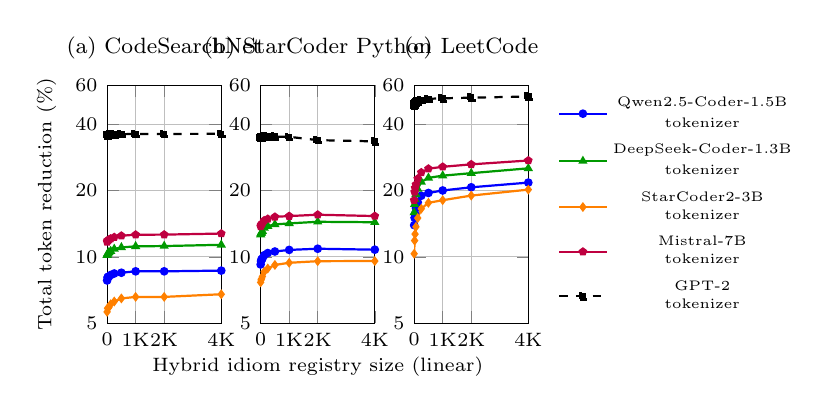
\begin{tikzpicture}
    \begin{groupplot}[
      group style={group size=3 by 1, horizontal sep=0.5cm},
      width=0.25\textwidth, height=4.6cm,
      xmin=0, xmax=4096,
      xtick={0,1024,2048,4096},
      xticklabels={0,1K,2K,4K},
      ymode=log,
      log basis y=10,
      ymin=5, ymax=60,
      ytick={5,10,20,40,60},
      yticklabels={5,10,20,40,60},
      grid=major,
      every axis plot/.append style={mark size=1.15pt},
      tick label style={font=\scriptsize},
      label style={font=\scriptsize},
      title style={font=\footnotesize},
      legend style={font=\scriptsize}
    ]
      \nextgroupplot[
        title={(a) CodeSearchNet},
        ylabel={Total token reduction (\%)},
        legend to name=capacitylegend,
        legend columns=1,
        legend style={font=\tiny, draw=none, inner sep=1pt, row sep=1pt}
      ]
      \addplot[blue, thick, mark=*] coordinates {(0,7.8077)(16,8.0515)(32,8.1152)(64,8.1254)(128,8.2675)(256,8.3972)(512,8.4647)(1024,8.5899)(2048,8.5903)(4096,8.6538)}; \addlegendentry{\shortstack{Qwen2.5-Coder-1.5B\\tokenizer}}
      \addplot[green!60!black, thick, mark=triangle*] coordinates {(0,10.1808)(16,10.3044)(32,10.3690)(64,10.4808)(128,10.6078)(256,10.8528)(512,11.0306)(1024,11.1555)(2048,11.1885)(4096,11.3350)}; \addlegendentry{\shortstack{DeepSeek-Coder-1.3B\\tokenizer}}
      \addplot[orange, thick, mark=diamond*] coordinates {(0,5.6213)(16,5.8406)(32,5.8406)(64,5.9011)(128,6.0912)(256,6.2676)(512,6.4703)(1024,6.5750)(2048,6.5753)(4096,6.7596)}; \addlegendentry{\shortstack{StarCoder2-3B\\tokenizer}}
      \addplot[purple, thick, mark=pentagon*] coordinates {(0,11.6817)(16,11.8695)(32,11.8695)(64,11.9508)(128,12.0962)(256,12.2760)(512,12.4615)(1024,12.5971)(2048,12.6095)(4096,12.7485)}; \addlegendentry{\shortstack{Mistral-7B\\tokenizer}}
      \addplot[black, thick, dashed, mark=square*] coordinates {(0,35.5275)(16,35.5962)(32,35.6663)(64,35.7265)(128,35.8212)(256,35.8974)(512,36.0377)(1024,36.1120)(2048,36.1223)(4096,36.1812)}; \addlegendentry{\shortstack{GPT-2\\tokenizer}}

      \nextgroupplot[title={(b) StarCoder Python}]
      \addplot[blue, thick, mark=*] coordinates {(0,9.2278)(16,9.5595)(32,9.7406)(64,9.8146)(128,10.1643)(256,10.3983)(512,10.5688)(1024,10.7461)(2048,10.8797)(4096,10.7711)};
      \addplot[green!60!black, thick, mark=triangle*] coordinates {(0,12.6086)(16,12.8037)(32,12.8798)(64,13.0623)(128,13.5165)(256,13.7892)(512,14.0235)(1024,14.1804)(2048,14.4184)(4096,14.3515)};
      \addplot[orange, thick, mark=diamond*] coordinates {(0,7.6560)(16,7.8561)(32,7.9468)(64,8.1439)(128,8.5467)(256,8.8476)(512,9.1840)(1024,9.3917)(2048,9.5514)(4096,9.5678)};
      \addplot[purple, thick, mark=pentagon*] coordinates {(0,13.7310)(16,13.9275)(32,14.0337)(64,14.2106)(128,14.6215)(256,14.8620)(512,15.1867)(1024,15.3075)(2048,15.5256)(4096,15.3093)};
      \addplot[black, thick, dashed, mark=square*] coordinates {(0,34.6694)(16,34.8084)(32,34.8612)(64,34.9797)(128,35.2898)(256,35.1541)(512,35.1359)(1024,35.0603)(2048,33.8584)(4096,33.4223)};

      \nextgroupplot[title={(c) LeetCode}]
      \addplot[blue, thick, mark=*] coordinates {(0,13.9227)(16,15.0363)(32,15.6538)(64,16.6486)(128,17.6669)(256,18.9342)(512,19.4923)(1024,20.0072)(2048,20.6804)(4096,21.7204)};
      \addplot[green!60!black, thick, mark=triangle*] coordinates {(0,15.8838)(16,17.3220)(32,18.2107)(64,19.2145)(128,20.3067)(256,21.8707)(512,22.8257)(1024,23.3562)(2048,23.9720)(4096,25.2205)};
      \addplot[orange, thick, mark=diamond*] coordinates {(0,10.3229)(16,11.8427)(32,12.6745)(64,13.6766)(128,14.9891)(256,16.5274)(512,17.5842)(1024,18.0711)(2048,18.9646)(4096,20.1828)};
      \addplot[purple, thick, mark=pentagon*] coordinates {(0,18.0617)(16,19.6943)(32,20.5342)(64,21.2864)(128,22.6276)(256,24.1537)(512,25.1173)(1024,25.6200)(2048,26.2876)(4096,27.3657)};
      \addplot[black, thick, dashed, mark=square*] coordinates {(0,48.4076)(16,49.1479)(32,49.6663)(64,50.1092)(128,50.7567)(256,51.5997)(512,52.1587)(1024,52.4306)(2048,52.7820)(4096,53.4191)};
    \end{groupplot}
    \node[anchor=west, font=\scriptsize] at ($(group c3r1.east)+(0.22cm,0)$) {\pgfplotslegendfromname{capacitylegend}};
    \node[font=\scriptsize] at ($(group c2r1.south)+(0,-0.55cm)$) {Hybrid idiom registry size (linear)};
  \end{tikzpicture}
  \vspace{-2pt}
  \vspace{-5pt}
  \caption{Registry-capacity curves across the three evaluation corpora and five model-associated tokenizers.}
  \Description{Three side-by-side line charts for CodeSearchNet, StarCoder Python, and LeetCode. Each chart plots total token reduction against a linear registry-size axis for the Qwen2.5-Coder-1.5B, DeepSeek-Coder-1.3B, StarCoder2-3B, Mistral-7B, and GPT-2 tokenizers. All curves rise most quickly at small registries and generally flatten as the registry grows.}
  \label{fig:capacity_curves}
\end{figure*}

These results establish two complementary sources of compression: Normalization removes deterministically recoverable structure, while Hybrid Idioms Shorthanding captures residual repetition on the normalized surface. The gains depend on the corpus and tokenizer, and the capacity curve shows rapidly diminishing returns as the registry grows. \paragraph{Answer to RQ1.} \tool provides compression across all evaluated combinations, with larger idiom gains on repetitive function-level code and stable normalization gains on heterogeneous repository code.

\subsection{RQ2: Dialect Learnability and Downstream Use}
\label{subsec:rq2}

Table~\ref{tab:rq2_absorption} reports the matched Baseline and \tool conditions for the
mainline Qwen2.5-Coder-1.5B experiment and three additional backbones. Each model
is evaluated on the same 164 HumanEval tasks under the same task protocol;
only the code surface differs between the two conditions. The Baseline condition
uses original Python, while \tool uses the calibrated dialect. \tool uses the complete
symmetric setting: both the model input and generated output follow the
calibrated dialect, and the generated program is restored to Python before
task evaluation.

\begin{table*}[!b]
    \centering
    \footnotesize
    \setlength{\tabcolsep}{5pt}
    \renewcommand{\arraystretch}{1.08}
    \caption{Pass@1 on the three downstream tasks for matched Baseline and \tool
    conditions. The Baseline condition uses original Python; the \tool condition
    uses the calibrated dialect. Every row uses the same 164 HumanEval tasks for
    the corresponding backbone.}
    \vspace{-5pt}
    \label{tab:rq2_absorption}
    \begin{tabular}{@{}llrrr@{}}
    \toprule
    \textbf{Model} & \textbf{Condition} & \textbf{Generation} & \textbf{Completion} & \textbf{Test generation} \\
    \midrule
    \multirow{2}{*}{Qwen2.5-Coder-1.5B} & Baseline & 43.90 & 85.00 & 33.00 \\
    & \tool & 42.07 & 83.00 & 36.00 \\
    \midrule
    \multirow{2}{*}{StarCoder2-3B} & Baseline & 31.10 & 28.05 & 71.95 \\
    & \tool & 29.27 & 34.15 & 98.17 \\
    \midrule
    \multirow{2}{*}{Mistral-7B} & Baseline & 27.44 & 26.22 & 98.17 \\
    & \tool & 12.80 & 27.44 & 97.56 \\
    \midrule
    \multirow{2}{*}{GPT-2} & Baseline & 0.00 & 23.17 & 0.00 \\
    & \tool & 0.00 & 22.56 & 1.83 \\
    \bottomrule
    \end{tabular}
    \vspace{2pt}
    \parbox{0.96\textwidth}{\footnotesize All entries are Pass@1 percentages. Baseline and \tool are compared within each backbone; the table is not intended to rank the base models. }
\end{table*}

Within-backbone comparisons show that StarCoder2-3B gains 6.10 points on completion and 26.22 points on test generation, while Qwen2.5-Coder-1.5B stays within 2.00 points on generation and completion and improves test generation by 3.00 points. Mistral-7B remains close on completion and test generation, whereas GPT-2 remains low in both conditions.

The dialect is learnable across backbones, with the clearest gains in repeated test-generation structures; completion is stable, while generation is more backbone-sensitive, especially for Mistral-7B.

\paragraph{Answer to RQ2.} Code models can learn and use the complete \tool dialect, which is competitive with the Baseline in most evaluated backbone--task combinations.

\subsection{RQ3: Effectiveness of Conditional Attention}
\label{subsec:rq3}

We first test whether Conditional Attention selects lower-shift occurrences before model adaptation. The scorer is fixed before evaluation, and the test problems do not overlap with its calibration problems.

Table~\ref{tab:conditional_attention_shift} compares policies at exactly the same reduction level: 400 tokens removed. Conditional Attention produces a cumulative suffix delta-NLL of $-5.03$, compared with $+2.65$ for 20,000 reduction-matched random selections. Reversing the learned ordering gives $+8.03$.

\begin{table}[H]
    \centering
    \small
    \setlength{\tabcolsep}{6pt}
    \renewcommand{\arraystretch}{1.08}
    \caption{Held-out representation shift at an equal reduction level. Each policy removes 400 tokens; lower delta-NLL is better.}
    \vspace{-5pt}
    \label{tab:conditional_attention_shift}
    \begin{tabular}{@{}lrr@{}}
    \toprule
    \textbf{Occurrence policy} & \textbf{Tokens removed (\#)} & \textbf{Delta-NLL} \\
    \midrule
    \textbf{Conditional Attention} & 400 & $\mathbf{-5.03}$ \\
    Matched random & 400 & $+2.65$ \\
    Reversed score & 400 & $+8.03$ \\
    \bottomrule
    \end{tabular}
\end{table}

At the same number of removed tokens, the difference is caused by the locations selected for compression rather than by the compression amount itself. This supports the claim that occurrence context matters and that a legal shorthand should not be materialized uniformly.

The fixed-point table isolates the ordering effect while holding the reduction amount constant. The following sweep varies the relative reduction level, and therefore the corresponding absolute token count, to test whether the same ordering remains useful across operating points.

Conditional Attention has lower delta-NLL than matched random selection at all four levels. Its largest advantage appears at 25--50\% of the available saving, while the 75\% setting remains favorable under aggressive compression.

\begin{table*}[!b]
  \centering
  \footnotesize
  \setlength{\tabcolsep}{5pt}
  \renewcommand{\arraystretch}{1.06}
  \caption{Reduction-level sweep for occurrence selection on the held-out split. ``Reduction (\%)'' is the relative fraction of all available candidate savings, while ``Tokens removed'' is its absolute token count. Each policy removes the same number of tokens within a row; lower delta-NLL is better. The random mean and standard deviation are computed from 20,000 matched selections.}
  \vspace{-5pt}
  \label{tab:conditional_attention_reduction_sweep}
  \begin{tabular}{@{}rrrrrr@{}}
  \toprule
  \textbf{Reduction (\%)} & \textbf{Tokens removed (\#)} & \textbf{Conditional Attention} &
  \textbf{Random mean $\pm$ std.} & \textbf{Difference} & \textbf{$z$} \\
  \midrule
  10\% & 160  & $-2.31$ & $1.07\ \pm\ 0.95$ & $-3.38$ & $-3.56$ \\
  25\% & 400  & $-5.03$ & $2.64\ \pm\ 1.37$ & $-7.67$ & $-5.61$ \\
  50\% & 800  & $-2.59$ & $5.30\ \pm\ 1.57$ & $-7.89$ & $-5.04$ \\
  75\% & 1200 & $3.47$  & $7.96\ \pm 1.37$ & $-4.49$ & $-3.29$ \\
  \bottomrule
  \end{tabular}
\end{table*}

The advantage is not tied to one hand-picked saving level. Conditional Attention improves the ordering of candidates across a range of reduction levels, although it does not remove the inherent cost of aggressive compression when most candidates are materialized.

To separate contextual scoring from registry frequency, we repeat the sweep
with controls that retain the same candidates and token-removal targets. The
global-pattern control ranks candidates without occurrence-level model
features; the reversed-score control reverses the learned ordering. At 25\%, the
Conditional Attention damage is $-5.03$, compared with $3.29$ for the global-pattern control
and $8.03$ for the reversed-score control. At 50\% the corresponding values are $-2.59$,
$5.06$, and $13.25$; at 75\% they are $3.47$, $8.15$, and $15.70$.

The mechanism is contextual rather than frequency-only. For a normalized sequence $a\ b\ c\ d$ with eligible pairs $ab$, $bc$, and $cd$, all three candidates are reversible, but if only $cd$ leaves the suffix NLL unchanged or lower, Conditional Attention selects $cd$ and leaves the others expanded. It therefore changes where a valid shorthand is materialized, not the registry or decoder.

Conditional Attention outperforms matched random selection at 10\%, 25\%, 50\%, and 75\% of the available shorthand saving and in all five problem-group folds. When comparisons are restricted to two occurrences of the same idiom, it ranks the lower-damage context first in 57.28\% of 3,195 pairs, compared with 50.06\% under within-idiom permutation. At the 25\% reduction level, fold-wise differences range from $-0.49$ to $-2.29$ NLL. Two folds reach the empirical $p<0.05$ threshold individually, while the remaining folds retain the same direction with fewer occurrences. A 500-trial label-shuffle control places the observed Conditional Attention score in the lower tail ($p=0.006$), and a within-pattern permutation test gives 57.28\% concordance versus a 50.06\% null rate ($p=0.002$).

We next measure the consequence for model adaptation. Conditional Attention and Random use the same initialization, optimizer, training-step count, and candidate registry; their packed training streams differ by only 0.43\% in token count. Figure~\ref{fig:conditional_attention_convergence} reports the mean validation curves across three runs. Conditional Attention has lower validation NLL at every one of the 11 checkpoints in every run. It reaches NLL below 1.0 at step 30, while Random does not reach the threshold within 100 steps. Across seeds, the final NLL difference is $-0.0398\pm0.0001$ and the area-under-learning-curve difference is $-3.97\pm0.02$ NLL--steps; Conditional Attention wins at every checkpoint in all three runs.

\begin{figure}[!t]
  \centering
  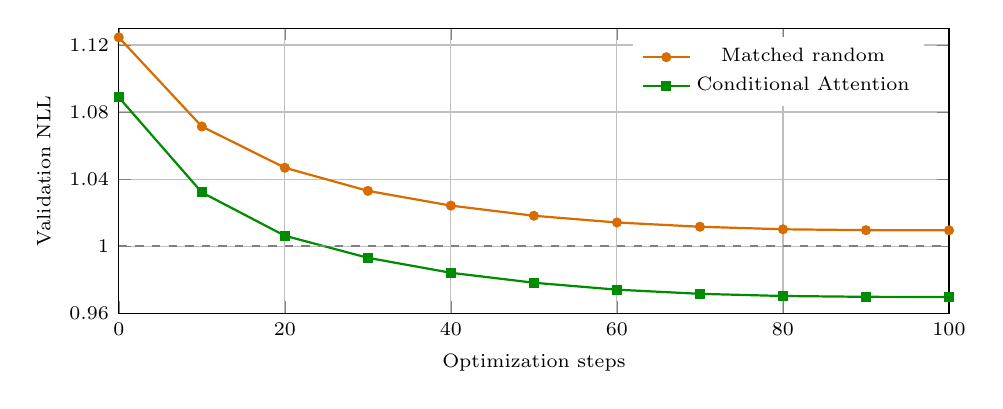
\begin{tikzpicture}
    \begin{axis}[
      width=\columnwidth,
      height=5.2cm,
      xmin=0, xmax=100,
      ymin=0.96, ymax=1.13,
      xtick={0,20,40,60,80,100},
      ytick={0.96,1.00,1.04,1.08,1.12},
      xlabel={Optimization steps},
      ylabel={Validation NLL},
      grid=major,
      tick label style={font=\scriptsize},
      label style={font=\scriptsize},
      legend style={font=\scriptsize, draw=none, at={(0.97,0.97)}, anchor=north east},
      every axis plot/.append style={thick, mark size=1.4pt}
    ]
      \addplot[orange!85!black, mark=*] coordinates {(0,1.12455)(10,1.07137)(20,1.04675)(30,1.03296)(40,1.02416)(50,1.01810)(60,1.01409)(70,1.01155)(80,1.01003)(90,1.00951)(100,1.00941)};
      \addlegendentry{Matched random}
      \addplot[green!55!black, mark=square*] coordinates {(0,1.08880)(10,1.03203)(20,1.00618)(30,0.99302)(40,0.98408)(50,0.97814)(60,0.97400)(70,0.97152)(80,0.97023)(90,0.96973)(100,0.96963)};
      \addlegendentry{Conditional Attention}
      \addplot[gray, dashed, no marks] coordinates {(0,1.0)(100,1.0)};
    \end{axis}
  \end{tikzpicture}
  \vspace{-5pt}
  \caption{Mean matched validation NLL across three adaptation runs. Conditional Attention reaches the fixed NLL threshold earlier and remains below Random throughout training.}
  \Description{A two-line convergence plot over 100 optimization steps. Conditional Attention remains below matched random selection at every checkpoint and crosses NLL 1.0 at step 30.}
  \label{fig:conditional_attention_convergence}
\end{figure}

\paragraph{Answer to RQ3.} At comparable compression, Conditional Attention selects lower-shift occurrences and yields faster, lower-loss adaptation.

\subsection{RQ4: Parameter Sensitivity}
\label{subsec:sensitivity}

Following the one-factor-at-a-time design used by REPFINDER~\cite{repfinder2021}, we vary one decision parameter while holding the others fixed. Because registry capacity determines the vocabulary used during adaptation, we select it on a held-out mixture of engineering code and algorithmic solutions that matches the adaptation domains. Its candidates are mined only from the corresponding training partitions, and the curve uses nested prefixes of one fixed ranking. The remaining mining-bound experiments use the held-out LeetCode split with the Qwen2.5-Coder-1.5B tokenizer and center on $f_{\min}=10$, $W_{\max}=8$, $H_{\max}=6$, and a registry cap of $K=800$; the larger cap prevents registry truncation from hiding differences among these parameters. No test split is used for parameter selection.

In Figure~\ref{fig:parameter_sensitivity}, $K$ is the registry capacity, namely
the maximum number of shorthand entries retained. The minimum support
$f_{\min}$ is the minimum number of occurrences required for a mined pattern
to remain a candidate. The maximum window $W_{\max}$ is the largest local
token or syntax window considered when collecting contiguous patterns. The
maximum captures $H_{\max}$ is the largest number of typed variable,
literal, or expression captures allowed in one generalized pattern. A plateau
means that increasing the parameter further produces negligible additional
token reduction under the fixed evaluation protocol.

\begin{figure*}[!t]
  \centering
  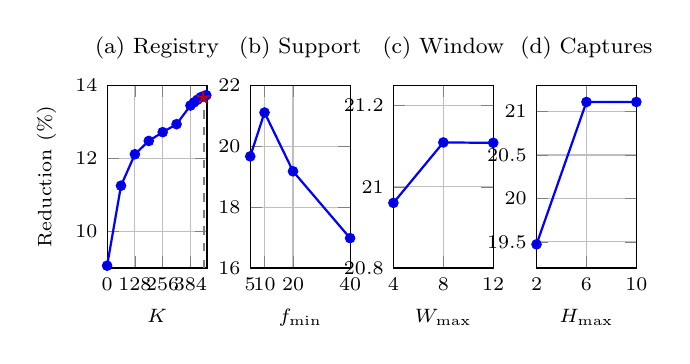
\begin{tikzpicture}
    \begin{groupplot}[
      group style={group size=4 by 1, horizontal sep=0.55cm},
      width=0.235\textwidth, height=3.9cm,
      grid=major,
      tick label style={font=\scriptsize},
      label style={font=\scriptsize},
      title style={font=\footnotesize},
      every axis plot/.append style={blue, thick, mark=*, mark size=1.5pt}
    ]
      \nextgroupplot[
        title={(a) Registry},
        xlabel={$K$}, ylabel={Reduction (\%)},
        xmin=0, xmax=460, ymin=9, ymax=14,
        xtick={0,128,256,384}
      ]
      \addplot coordinates {(0,9.0629)(64,11.2531)(128,12.1151)(192,12.4793)(256,12.7194)(320,12.9382)(384,13.4493)(400,13.5346)(416,13.6067)(432,13.6788)(448,13.7150)(457,13.7312)};
      \addplot[gray, dashed, no marks] coordinates {(448,9)(448,14)};
      \addplot[red!75!black, only marks, mark=star, mark size=2.3pt] coordinates {(443,13.6605)};

      \nextgroupplot[
        title={(b) Support},
        xlabel={$f_{\min}$},
        xmin=5, xmax=40, ymin=16, ymax=22,
        xtick={5,10,20,40}
      ]
      \addplot coordinates {(5,19.6677)(10,21.1094)(20,19.1765)(40,16.9805)};

      \nextgroupplot[
        title={(c) Window},
        xlabel={$W_{\max}$},
        xmin=4, xmax=12, ymin=20.8, ymax=21.25,
        xtick={4,8,12}
      ]
      \addplot coordinates {(4,20.9604)(8,21.1094)(12,21.1085)};

      \nextgroupplot[
        title={(d) Captures},
        xlabel={$H_{\max}$},
        xmin=2, xmax=10, ymin=19.2, ymax=21.3,
        xtick={2,6,10}
      ]
      \addplot coordinates {(2,19.4716)(6,21.1094)(10,21.1094)};
    \end{groupplot}
  \end{tikzpicture}
  \vspace{-5pt}
  \caption{One-factor sensitivity of Hybrid Idioms Shorthanding. Registry capacity $K$, minimum support $f_{\min}$, maximum window $W_{\max}$, and maximum captures $H_{\max}$ are defined in the text. Panel (a) uses the held-out adaptation-domain mixture; the star marks the 443-entry training registry obtained by pruning the 448-entry plateau vocabulary. Panels (b)--(d) use held-out LeetCode.}
  \Description{Four line charts show token reduction against registry capacity, minimum pattern support, maximum mining-window length, and maximum number of typed captures. The registry curve approaches a plateau near 448 entries and marks the deployed 443-entry registry; reduction peaks at support 10 and plateaus at window 8 and capture bound 6.}
  \label{fig:parameter_sensitivity}
\end{figure*}

Figure~\ref{fig:parameter_sensitivity}(a) makes the capacity plateau explicit. Total reduction rises from 9.06\% without idiom entries to 13.45\% at $K=384$, then reaches 13.53\%, 13.61\%, and 13.68\% at $K=400$, 416, and 432. Expanding the registry to 448 and then to the complete 457-candidate vocabulary yields only 13.715\% and 13.731\%, respectively. Thus $K=448$ retains 99.65\% of the maximum shorthand gain, while the final nine entries contribute only 0.016 percentage points. For adaptation, we further remove five entries that are not materialized in at least one of the actual training or validation corpora. The resulting $K=443$ registry retains 98.49\% of the maximum shorthand gain; all 443 symbols occur in the adaptation training corpus, with a median of 56 occurrences and 430 symbols appearing at least ten times.

The mining bounds have clearer interior optima. Setting $f_{\min}=10$ gives 21.11\% reduction, compared with 19.67\%, 19.18\%, and 16.98\% at 5, 20, and 40. Increasing $W_{\max}$ from 4 to 8 improves reduction from 20.96\% to 21.11\%, with no further gain at 12. Likewise, increasing $H_{\max}$ from 2 to 6 improves reduction from 19.47\% to 21.11\%, while 10 produces the same result.

The sensitivity results identify an operating region rather than a universally optimal value. Registry capacity and minimum pattern support have the largest effect, while the window and capture bounds reach an early plateau. We therefore use $(K,f_{\min},W_{\max},H_{\max})=(443,10,8,6)$, which preserves nearly all available compression while avoiding unnecessary vocabulary entries and mining cost.

\paragraph{Answer to RQ4.} \tool is most sensitive to registry capacity and minimum pattern support, while the window and capture bounds enter a stable plateau. Capacity saturates at approximately 448 entries, and exposure-aware pruning produces the 443-entry registry used for mainline adaptation.

\subsection{Ablation Study}
\label{subsec:ablation}

We ablate \tool at its two principal decision boundaries: what is represented compactly by the codec, and where an eligible shorthand is materialized.

\begin{table}[H]
    \centering
    \footnotesize
    \setlength{\tabcolsep}{4pt}
    \renewcommand{\arraystretch}{1.08}
    \caption{Codec-component ablation across the five tokenizers. Values are token-reduction ranges; the Hybrid column reports the additional gain over Normalization.}
    \vspace{-5pt}
    \label{tab:codec_ablation}
    \begin{tabular}{@{}lrrr@{}}
    \toprule
    \textbf{Corpus} & \textbf{Normalization (\%)} & \textbf{Hybrid gain (pp)} & \textbf{Full \tool (\%)} \\
    \midrule
    CodeSearchNet & 5.62--35.53 & +0.58--0.98 & 6.57--36.11 \\
    StarCoder Python & 7.66--34.67 & +0.35--1.69 & 9.35--35.02 \\
    LeetCode & 10.32--48.41 & +4.52--8.81 & 19.13--52.93 \\
    \bottomrule
    \end{tabular}
\end{table}

Table~\ref{tab:codec_ablation} shows that Normalization alone provides the larger and more stable part of the reduction. Adding Hybrid Idioms Shorthanding produces a positive gain for every tokenizer, with the largest contribution on LeetCode. Holding the candidate registry and token-removal level fixed, replacing Conditional Attention with matched random occurrence selection changes cumulative delta-NLL from $-5.03$ to $+2.65$; reversing the learned ordering further increases it to $+8.03$. The final validation NLL rises from 0.9696 with Conditional Attention to 1.0094 with matched random selection, and the random policy does not reach the fixed NLL threshold within the 100-step training run.

The ablation results show that the components address different sources of difficulty. Normalization supplies broadly available structural reduction, Hybrid Idioms Shorthanding captures residual corpus repetition, and Conditional Attention reduces the learning cost introduced by deciding where those idioms are materialized. The three components are complementary rather than interchangeable.


\subsection{Threats and Limitations}

\hspace*{\parindent}\textbf{Threats.} To reduce data leakage, we construct the mining,
calibration, training, validation, and test partitions independently and check
for overlap at the problem-group level. Residual semantic duplication across
independently sourced corpora may nevertheless remain. Our codec measurements
depend on the correctness of the parser, tokenizer integrations, and inverse
transformations; we mitigate this threat with round-trip tests and by counting
fallback inputs in the reported coverage rather than silently excluding them.
Downstream pass rates may vary with training seed and checkpoint selection. We
therefore use a fixed evaluation protocol and report the checkpoint and
condition used for each comparison; broader multi-seed training would further
strengthen these results. Finally, the evaluated corpora, Python syntax, and
model families do not cover every programming language or deployment setting,
so the observed reduction and adaptation behavior should not be assumed to
transfer unchanged beyond the studied configurations.

\indent\textbf{Limitations.} The main codec guarantee is AST-equivalent executable recovery for accepted outputs, not byte-for-byte preservation of formatting or comments. Some inputs still fall back to native Python and remain in the denominator when reporting coverage. RQ1 uses tokenizer- and corpus-specific registries, so it measures capacity rather than universal cross-domain transfer. RQ2 now includes several model families and sizes, but the parallel runs use model-specific adapters and should be interpreted as within-backbone comparisons rather than a ranking of base models. RQ3 uses a fixed candidate subset from one primary calibration domain. Offline attention scoring also adds a preprocessing cost. Future evaluation should test whether the same selection principle transfers to additional programming languages and longer-context tasks.

% !TeX root = ../main.tex

\section{Related Work}
\label{sec:related}


\textbf{Token Reduction.} Prior work has shortened code inputs by removing or rewriting elements judged less important. DietCode, SlimCode, and LeanCode use model importance, program structure, or code naturalness to guide such simplification~\cite{dietcode2022,slimcode2024,leancode2025}; program-minimization studies similarly seek smaller inputs that preserve a prediction or expose model behavior~\cite{p2im2021,rabin2021,rabin2022}. These methods primarily target task-preserving or lossy reduction, rather than exact source-level recovery. Reversible methods instead define a compact representation that can be deterministically converted back to standard code. SimPy redesigns the Python surface grammar to remove layout and delimiter redundancy~\cite{simpy2024}, whereas TokenSugar mines recurring patterns and maps them to single-token shorthands~\cite{tokensugar2024}. Our work combines these two reduction levels and additionally studies whether a model-derived signal should decide where an otherwise valid shorthand is materialized.

This pattern-based direction is related to code-idiom mining, which extracts recurring AST, graph, or programmatic structures for abstraction, language design, or structured generation~\cite{allamanis2014,allamanis2018mining,sivaraman2022,iyer2019,shin2019}. NormCoRe differs in treating mined idioms as part of a reversible model-facing dialect: captures preserve occurrence-specific identifiers and expressions, while the decoder maintains the inverse mapping. The goal is therefore not only to find frequent idioms, but to select compact forms that remain valid, learnable, and recoverable.
This requirement is stricter than ordinary source simplification because a generated shorthand must remain well-formed under the same fixed registry and must be expanded without relying on a human repair step.

SimPy and TokenSugar also differ in how their compact forms are obtained. SimPy relies primarily on a human-designed grammar whose structural conventions are shared across inputs, whereas TokenSugar fixes a corpus-mined shorthand vocabulary and matching policy before model adaptation. This distinction creates a representation-learning question: a shorthand can be legal and token-efficient while still replacing cues that a model uses for prediction. NormCoRe therefore treats compression validity and occurrence selection as separate decisions. Normalization and Hybrid Idioms Shorthanding define the reversible candidate space; Conditional Attention decides whether an eligible occurrence should be materialized in shorthand form.

\textbf{Code Encoding and Model-Aware Representation.} Code models use subword tokenization and, in some cases, explicit identifier or program-structure signals~\cite{sennrich2016,karampatsis2020,wang2021,feng2020,guo2021,guo2022}. These methods improve code representation but do not primarily remove Python layout redundancy while providing a deterministic inverse codec. Interpretability studies investigate whether attention captures code syntax, data flow, or semantic structure~\cite{chen2022cat,wan2022,karmakar2021,bui2019,ma2022}. Model-aware prompt compression also shows that internal signals can guide input selection, although it targets general natural-language prompts and may discard information~\cite{llmlingua2023}. \tool extends this idea to reversible code representation: Conditional Attention uses contextual model evidence to select among legal shorthand occurrences without discarding the information required for restoration.

\textbf{Large Language Models for Generative Software Engineering.} Code completion, generation, testing, repository-level completion, and issue resolution require outputs that satisfy syntax, scope, interface, and execution constraints~\cite{raychev2014,chen2021codex,lemieux2023codamosa,liu2023repobench,jimenez2024swebench}. Repository-level tasks may additionally depend on definitions and usage examples distributed across files. A compact representation for these settings must therefore remain learnable and generatable while decoding deterministically to executable code; deleting a declaration or identifier can break cross-location dependencies even when a task's immediate prediction is preserved. Accordingly, \tool separates codec-side compression capacity from dialect learnability and evaluates whether model-informed occurrence selection improves the trade-off between reduction and downstream capability.

% \section{Discussion}

\subsection{What the Results Establish}

The experiments separate three properties that are often conflated in compact code representations. First, the representation has measurable compression capacity: Normalization removes recoverable layout and structural redundancy, while Hybrid Idioms Shorthanding adds corpus- and tokenizer-dependent savings on the normalized surface. Second, a model can learn the resulting dialect and use it in generation, completion, and test generation while remaining close to its Baseline condition on original Python. Third, reversible recovery does not imply that every compact representation is equally easy for a model to learn, which motivates model-informed occurrence selection.

RQ3 evaluates this selection view at matched reduction levels. On held-out occurrences, Conditional Attention changes cumulative suffix NLL by $-5.03$, compared with $+2.65$ for matched random selection. Across three adaptation runs, it remains below Random throughout training, reaches NLL below 1.0 by step 30, and finishes at 0.9696 rather than 1.0094. The signal is computed before materializing the dialect, so it does not modify the model's autoregressive generation loop.

\subsection{Domain and Tokenizer Dependence}

Hybrid Idioms Shorthanding is data-driven, so its gain follows the repetition structure of the target corpus and the token boundaries of the chosen tokenizer. LeetCode contains compact, repeated algorithmic idioms and therefore yields larger shorthand gains than the more heterogeneous CSN and StarCoder Python corpora. The positive gains on all three corpora show that idiom collection can absorb residual patterns across both function-level and repository-level code while adapting its registry to the target distribution.

\section{Conclusion}

We presented \tool, a reversible representation for Python code that combines grammar-aware Normalization with multi-granularity Hybrid Idioms Shorthanding. The codec reduces recoverable structural and recurring-pattern redundancy while retaining the information needed to restore executable Python. Across corpora and tokenizers, the two components provide complementary reductions with diminishing returns as the registry grows, and adapted code models can learn and use the resulting dialect across the evaluated generation, completion, and test-generation tasks. Conditional Attention further selects eligible shorthand occurrences using a model-derived contextual signal, reducing representation shift and adaptation cost at matched compression levels. Together, these results support reversible, model-aware code representation as a practical direction for token-efficient code processing.

\section{Data Availability}

We provide our anonymized artifact, including the codec implementation,
evaluation scripts, and configuration files, at
\url{https://github.com/BluesOctopus/NormCoRe.git}.


\bibliographystyle{ACM-Reference-Format}
\bibliography{references}

\end{document}
